%%%%%%%%%%%%%%%%%%%%%%%%%%%%%%%%%%%%%%%%%%%%%%%%%%%%%%%%%%%%%%%%%%%%%%%%%%%%%%%
%                     University of Glasgow Thesis Template  
%   Created by : Majed Al Saeed
%   Date:        Feb 2014
%   Department of Computer Science
%   University of Glasgow
%   email: maj.saeed@gmail.com
%
%%%%%%%%%%%%%%%%%%%%%%%%%%%%%%%%%%%%%%%%%%%%%%%%%%%%%%%%%%%%%%%%%%%%%%%%%%%%%%%

\documentclass[a4paper,12pt]{report}
% Macros.tex
% created: June 4 2012
% Majed Al Saeed
%
%%%%%%%%%%%%%%%%%%%%%%%%%%%%%%%%%%%%%%%%%%%%%%%%%%%%%%%%%%%%%%%%%%%%%%%%%%%%%%%


% abbreviations
\newcommand{\ie}{i.e.\xspace}
\newcommand{\eg}{e.g.\xspace}
\newcommand{\Fex}{For example,\xspace}
\newcommand{\fex}{for example,\xspace}
\newcommand{\Fin}{For instance,\xspace}
\newcommand{\fin}{for instance,\xspace}
\newcommand{\Sas}{Such as\xspace}
\newcommand{\sas}{such as\xspace}
\newcommand{\cf}{cf.\xspace}
\newcommand{\Cf}{Cf.\xspace}
\newcommand{\wrt}{w.\,r.\,t.\xspace}
\newcommand{\Wrt}{W.\,r.\,t.\xspace}
\newcommand{\wlg}{w.\,l.\,o.\,g.\xspace}
\newcommand{\Wlg}{W.\,l.\,o.\,g.\xspace}
\newcommand{\resp}{resp.\xspace}
\newcommand{\etc}{etc.\xspace}
\newcommand{\etal}{et~al.~}

% names

\newcommand{\ghc}{GHC}
\newcommand{\ghcf}{Glasgow Haskell Compiler}







%==============================title page info=================================

% Name of the author
\newcommand{\auth}{FName LName}   
% Title of Thesis                
\newcommand{\thesistitle}{Thesis Title}
% Degree  
\newcommand{\degree}{Doctor of Philosophy} 
% Date submitted
\newcommand{\supdate}{September 2014}


%===================================packages===================================
\usepackage[top=18mm, bottom=18mm, left=40mm, right=15mm]{geometry}
\usepackage{setspace}
\usepackage{fancyhdr}
\usepackage[citecolor=black, urlcolor=black,
  linkcolor=black, colorlinks=true, bookmarksopen=false, bookmarks=true]{hyperref}
\usepackage[toc,nonumberlist]{glossaries}
%Glossaries
\makeglossaries

% You must define terms or symbols before you can use them in the document. This is best done in the preamble. Each term is defined using:
% 
% \newglossaryentry{<label>}{<settings>}
% 
% where <label> is a unique label used to identify the term. The second argument, <settings>, is a key=value comma separated list that is used to set the required information for the term. A full list of available keys can be found in "Defining Glossary Entries" in the main glossaries user manual. The principle keys are name and description.
% 
% For example, to define the term "electrolyte":
% 
% \newglossaryentry{electrolyte}{name=electrolyte,
% description={solution able to conduct electric current}}
% 
% In the above example, the label and the name happen to be the same. In the next example, the name contains a ligature but the label doesn't:
% 
% \newglossaryentry{oesophagus}{name=\oe sophagus,
% description={canal from mouth to stomach},
%plural=\oe sophagi}

%\newacronym{<label>}{<abbrv>}{<full>}

%\gls{<label>}
%\glspl{<label>}


\newacronym{ghcsmp}{GHC-SMP}{Haskell on a Shared Memory Multiprocessor}


\newacronym{pe}{PE}{Processing Element}



%\newacronym{}{}{}




\usepackage{graphicx}
\usepackage{subfigure}
\usepackage{xspace}
\usepackage{listings}
\usepackage{pdfpages}
\usepackage{alltt}
\usepackage{float} % to use [H] 
\usepackage[notindex, nottoc, notlof, notlot ]{tocbibind} 

\usepackage{lscape}    % if you want to use land scape in one paper 
                       %...\begin{landscape}\end{landscape}

% thesw 2 lines if you like to see deep contents
%\setcounter{tocdepth}{3}   
\setcounter{secnumdepth}{3}


\usepackage{listings}
\lstset{ %
language=Haskell,                % choose the language of the code
basicstyle=\scriptsize,       % the size of the fonts that are used for the code
numbers=left,                   % where to put the line-numbers
numberstyle=\scriptsize,      % the size of the fonts that are used for the line-numbers
stepnumber=1,                   % the step between two line-numbers. If it is 1 each line will be numbered
numbersep=5pt,                  % how far the line-numbers are from the code
backgroundcolor=\color{white},  % choose the background color. You must add \usepackage{color}
showspaces=false,               % show spaces adding particular underscores
showstringspaces=false,         % underline spaces within strings
showtabs=false,                 % show tabs within strings adding particular underscores
frame=lines,           % adds a frame around the code, single
tabsize=2,          % sets default tabsize to 2 spaces
captionpos=t,           % sets the caption-position to bottom
breaklines=true,        % sets automatic line breaking
breakatwhitespace=false,    % sets if automatic breaks should only happen at whitespace
%keywordstyle=\color{blue},          % keyword style
%commentstyle=\color{green},       % comment style
%stringstyle=\color{mauve},         % string literal style
escapeinside={\%*}{*)}          % if you want to add a comment within your code
}

%===================================Document===================================
\begin{document}
\begin{spacing}{1.5}

%==================================Title page==================================
\pagenumbering{arabic}
\pagestyle{empty}
\begin{center}
\begin{spacing}{2}
{\large{\ \\  \vspace{1.5cm}\textbf{\MakeUppercase{\thesistitle}}}}\\
\end{spacing}
\vfill
%{\Large\textit{by}}\\\vspace{0.2cm}
{\Large\upshape{\auth}}\\\vspace{2.0cm}
{\large Submitted in Fulfilment of the Requirements for the Degree of \\ \degree}\\
\vspace{1cm}

\includegraphics[width=3cm]{Front/Figures/Logo.png}\\
\vspace{0.5cm}
{\large\textsc{University of Glasgow}\\
\textsc{College of Science and Engineering}\\
\textsc{School of Computing Science}}\vfill
{\large{\supdate}}
\end{center}
{\small The copyright in this thesis is owned by the author. Any quotation from the thesis or use of any of the information contained in it must acknowledge this thesis as the source of the quotation or information.}
%==================================frontmater==================================
\clearpage
\pagestyle{plain}
\noindent
{\LARGE\textbf{Abstract}}

\vspace{0.5cm}

\begin{spacing}{1.03} 
\noindent
Write abstract here..

\end{spacing}
\newpage
\noindent
{\LARGE\textbf {Dedication}}

\vspace{9cm}

\begin{spacing}{1} 
\noindent

\begin{center}
To my Mother and Father.
\end{center}

\end{spacing}
\newpage
\noindent
{\LARGE\textbf{Acknowledgements}}
\vspace{1cm}

\begin{spacing}{1.5} 
\noindent
Write here...

\end{spacing}

\newpage
\noindent
{\LARGE\textbf{Declaration}}
\vspace{1cm}

\begin{spacing}{1.5} 
\noindent
I declare that, except where explicit reference is made to the contribution of others, that this dissertation is the result of my own work and has not been submitted for any other degree at the University of Glasgow or any other institution.





\vspace{3cm}
\begin{flushright}
Write your name here
\end{flushright}
\end{spacing}
\newpage
\tableofcontents
\listoftables
\listoffigures

%===================================headings===================================
\clearpage
\pagestyle{fancy}
\fancyhead{}
\lhead{\slshape \leftmark}  
\cfoot{\thepage}
\renewcommand{\headrulewidth}{0.4pt}
\renewcommand{\footrulewidth}{0.0pt}
\renewcommand{\chaptermark}[1]{\markboth{\chaptername\ \thechapter. \ #1}{}}
%===================================Chapters===================================


                             
\chapter{Introduction}
\label{ch:introduction}


\section{Context}



How to use Macros. The \ghcf{} (\ghc) is write.

How to cite. According to Akhter and Roberts \cite{Akhter06} write.
According to Shende \etal\cite{Shende98-TAU} write.


How to use glossaries. The number of \glspl{pe} write.
The \gls{ghcsmp} is write.




\section{Thesis Statement}



\section{Contributions}



\begin{enumerate}


\item 
\textbf{Write.}.  
detail here.


\item 
\textbf{Write.}.  
detail here.

\end{enumerate}




\section{Authorship and Publications}








\section{Thesis Structure}

The structure of this thesis is as follows:

\textbf{Chapter~\ref{ch:Background}} \space gives....




\chapter{Background}
\label{ch:Background}

\section{Introduction}




\section{Parallel Architectures}

\begin{figure}[H]
\begin{center}
 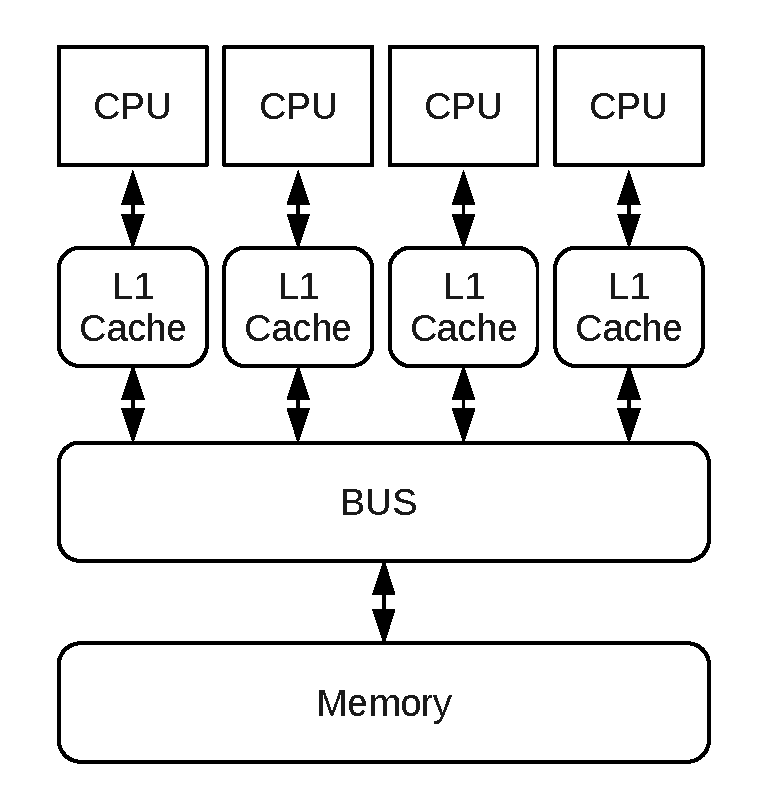
\includegraphics [width=6cm]{Background/Figures/shared-memory-SMP.pdf}
 \caption{Shared Memory SMP Architecture}
 \label{fig:shared-memory-SMP}
\end{center}
\end{figure}

\section{Summary}





\chapter{Conclusion and Future Work}
\label{ch:Conclusion}


\section{Summary}


\section{Limitations}


\section{Future Work}






%===================================Appendix===================================
\appendix
\renewcommand{\chaptermark}[1]{\markboth{Appendix \thechapter. \ #1}{}}

\chapter{Benchmarks}
\label{ch:Benchmarks}







\vspace{3mm}
\begin{spacing}{1} 
\lstinputlisting[
language=Haskell,
caption=Fibonacci Benchmark Implementation., 
label=ls:fib_benchmark_implementation, 
%float
]{Benchmarks/Code/HdpH_Fib.hs}
\end{spacing}



\section{Sum Euler}
\label{se:sumEuler_benchmark_imp}

\vspace{3mm}
\begin{spacing}{1} 
\lstinputlisting[
language=Haskell,
caption=Sum Euler Benchmark Implementation., 
label=ls:sumEuler_benchmark_implementation, 
%float
]{Benchmarks/Code/HdpH_SumEuler.hs}
\end{spacing}


%==================================glossaries==================================
% In order for the glossaries to appear you should run this command 
% on the terminal $ makeglossaries Thesis
\printglossaries

%=================================Bibliography=================================
\bibliographystyle{abbrv}
\bibliography{BIBLIOGRAPHY}

\end{spacing}
\end{document}


